


		section{Dynamical Aspects}
			\subsubsection{Time Evolution of $\ket{\psi(t)}$}
				After the static case we now want to investigate the dynamical properties of the two-state system. We calculate the time evolution of $\ket{\psi(t)} = \left(\begin{array}{cc} a_1(t) & a_2(t)\end{array}\right)^T$ with the Schrödinger equation and the perturbed Hamiltonian \eqref{eq:perturbedhamiltonian}:
				\begin{align}
					i\hbar \diff{}{t}\ket{\psi(t)}&=\left(\hat{H}+\hat{W}\right)\ket{\psi(t)},\\
					i\hbar \diff{}{t}\left(\begin{array}{c} a_1(t) \\ a_2(t) \end{array}\right) &= \left( \begin{array}{cc} \tilde{E}_1 & W_{12} \\ W_{12}^* & \tilde{E}_2 \end{array} \right) \left(\begin{array}{c} a_1(t) \\ a_2(t) \end{array} \right).
				\end{align}
				For the state $\ket{\psi(t)}$ we get
				\begin{align}
					\ket{\psi(t)}=\lambda \eexp{-i{E_+}t/{\hbar}} \ket{\psi_+} + \mu \eexp{-i{E_-}t/{\hbar}} \ket{\psi_-} \label{eq:psitimeevolution}
				\end{align}
				with the factors $\lambda$ and $\mu$.

				If we start in the state $\ket{\varphi_1}$, what is the probability
				\begin{align}
					P_2(t)=\left|\braket{\varphi_2|\psi(t)}\right|^2
				\end{align}
				to find the system in the state $\ket{\varphi_2}$? As a first step, we have to apply the initial condition to \eqref{eq:psitimeevolution} and express $\ket{\varphi}$ in terms of \eqref{eq:staticpsiplus} and \eqref{eq:staticpsiminus}:
				\begin{align}
					\ket{\psi(0)} \overset{!}{=}& \ket{\varphi_1}\\
											  = & \eexp{i{\varphi}/{2}} \left[ \cos\left( \frac{\theta}{2}\right) \ket{\psi_+}-\sin\left(\frac{\theta}{2}\right)\ket{\psi_-}\right]
				\end{align}
				By equating the coefficients we get for $\lambda$ and $\mu$:
				\begin{align}
					\lambda = \eexp{i{\varphi}/{2}}\cos\left(\frac{\theta}{2}\right), \qquad  \mu = -\eexp{i{\varphi}/{2}}\sin\left(\frac{\theta}{2}\right).
				\end{align}
				One thus gets:
				\begin{align}
					\hspace{-2mm} P_2(t)	=&\left|\braket{\varphi_2|\psi(t)}\right|^2 \\
											=& \left|\eexp{i\varphi} \sin\left(\frac{\theta}{2}\right)\cos\left(\frac{\theta}{2}\right)\left[\eexp{-i{E_+}t/{\hbar}} - \eexp{-i{E_-}t/{\hbar}}\right]\right|^2\\
											=& \sin^2(\theta)\sin^2\left(\frac{E_+-E_-}{2\hbar}t\right)
				\end{align}
				$P_2(t)$ can be expressed with $\Delta$ and $W_{12}$ alone. The obtained relation is called Rabi's formula:
				\begin{align}
					\Aboxed{P_2(t)=\frac{1}{1+\left(\frac{\Delta}{|W_{12}|}\right)^2}\sin^2\left(\sqrt{|W_{12}|^2+\Delta^2}\frac{t}{\hbar}\right)}
				\end{align}

				\begin{figure}
					\begin{center}
						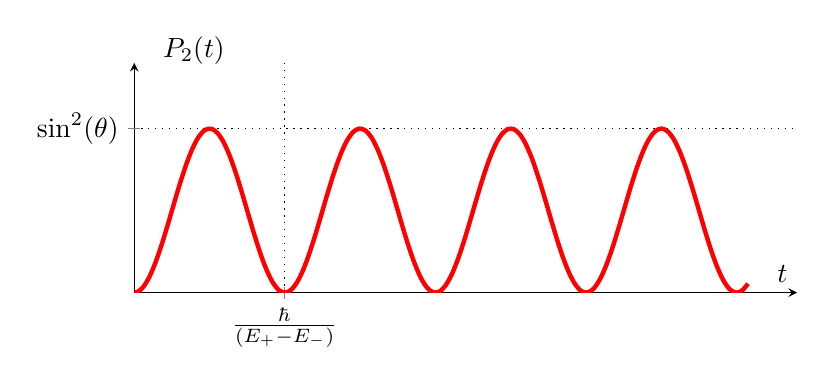
\begin{tikzpicture}
							\begin{axis}
							[
								axis x line=middle,
								axis y line=left,
								xmin = 0, xmax = {5.4},
								ymin = 0, ymax = {1.4},
								samples=200,
								xlabel=$t$,
								y label style={at={(axis description cs:0.09,.95)},rotate=-90,anchor=south},
								ylabel = $P_2(t)$,
								xtick = \empty,
								ytick = \empty,
								height = 4.5cm,
								width = 10cm,
								extra x ticks = {1.225},
								extra y ticks = {1},
								extra tick style={grid=major, grid style={line width = 0.5pt, dotted, black}},
								extra x tick labels={$\frac{\hbar}{(E_+-E_-)}$},
								extra y tick labels={$\sin^2(\theta)$},
							]
							\addplot[mark=none, ultra thick, smooth, color=red] expression {(sin(46.7*x*pi))^2};
							\end{axis}
						\end{tikzpicture}
						\caption{Rabi oscillations}
					\end{center}
				\end{figure}